% Defensa oral · TPI Decision Intelligence Capstone (EAyMR 2026, UCA)
% Compilar con LuaLaTeX (dos pasadas):  lualatex slides_defensa.tex
% Fuentes: Cambria (títulos) y Calibri (texto), incluidas en Windows.
% Los gráficos de fig/*.pdf se regeneran con scripts/figs.py; las capturas de la app, con scripts/shots.py.
\documentclass[aspectratio=169,10pt]{beamer}

\usepackage{fontspec}
\usepackage{unicode-math}
\setsansfont{Calibri}
\newfontfamily\headfont{Cambria}[BoldFont={Cambria Bold},ItalicFont={Cambria Italic}]
\setmonofont{Consolas}[Scale=0.88]
\setmathfont{Cambria Math}
\usepackage[spanish,es-noshorthands,es-nodecimaldot]{babel}
\usepackage{graphicx,booktabs,tabularx,ragged2e}
\usepackage{tikz}
\usetikzlibrary{arrows.meta,positioning,calc}
\graphicspath{{fig/}}

% ---------------------------------------------------------------- paleta
\definecolor{ink}{HTML}{1B2A2F}      % texto y fondos oscuros
\definecolor{deep}{HTML}{24474A}     % fondo de portada y cierre
\definecolor{deepcard}{HTML}{2F5A5E}
\definecolor{tint}{HTML}{EEF3F2}     % tarjetas claras
\definecolor{muted}{HTML}{56666A}
\definecolor{coral}{HTML}{D9482B}    % causal (What-If)
\definecolor{teal}{HTML}{22706B}     % predictivo (What-Is)
\definecolor{amber}{HTML}{C9821B}    % proceso y app
\definecolor{slate}{HTML}{4F5F86}    % datos e inferencia
\definecolor{okgreen}{HTML}{2E9E5B}
\colorlet{titlecol}{ink}
\colorlet{msgcol}{muted}
\colorlet{cardfill}{tint}
\colorlet{cardtitle}{ink}
\colorlet{cardtext}{ink}

% ---------------------------------------------------------------- plantilla
\setbeamertemplate{navigation symbols}{}
\setbeamersize{text margin left=8mm,text margin right=8mm}
\setbeamercolor{normal text}{fg=ink}
\setbeamerfont{normal text}{size=\small}
\newcommand{\pillcolor}{slate}
\newcommand{\pilltext}{}
\newcommand{\pill}[2]{\renewcommand{\pillcolor}{#1}\renewcommand{\pilltext}{#2}}
\setbeamertemplate{frametitle}{%
  \vspace{4.2mm}%
  \begin{tikzpicture}[remember picture,overlay]
    \node[anchor=north east,fill=\pillcolor,text=white,rounded corners=1.6mm,
          inner xsep=2.4mm,inner ysep=1.1mm,font=\scriptsize\bfseries]
      at ([xshift=-8mm,yshift=-4.6mm]current page.north east) {\pilltext};
  \end{tikzpicture}%
  \parbox[t]{112mm}{\RaggedRight\hyphenpenalty=10000 \headfont\Large\bfseries\color{titlecol}\insertframetitle}\par
  \vspace{0.9mm}%
  {\footnotesize\itshape\color{msgcol}\insertframesubtitle}\par
  \vspace{-0.6mm}}
\setbeamertemplate{footline}{%
  \hspace{8mm}{\tiny\color{msgcol}Decision Intelligence Capstone · EAyMR 2026 · UCA · Grupo Átomos}%
  \hfill{\tiny\color{msgcol}\insertframenumber\,/\,\inserttotalframenumber}\hspace{8mm}\vspace{3.2mm}}
\newenvironment{darkslide}{%
  \begingroup
  \setbeamercolor{background canvas}{bg=deep}%
  \setbeamercolor{normal text}{fg=white}\usebeamercolor[fg]{normal text}%
  \colorlet{titlecol}{white}\colorlet{msgcol}{white!78!deep}%
  \colorlet{cardfill}{deepcard}\colorlet{cardtitle}{white}\colorlet{cardtext}{white!92!deep}%
}{\endgroup}

% ---------------------------------------------------------------- piezas
\newcommand{\nosp}{\spaceskip0pt\xspaceskip0pt\RaggedRight\hyphenpenalty=10000 }
% \card[color del título]{ancho}{título}{cuerpo}            (alto natural)
\newcommand{\card}[4][cardtitle]{%
  \begin{tikzpicture}[baseline=(c.north)]
    \node[rounded corners=1.8mm,fill=cardfill,inner sep=2.4mm,anchor=north west] (c)
      {\begin{minipage}[t]{#2}\nosp
         {\small\bfseries\color{#1}#3\par}\vspace{0.5mm}{\footnotesize\color{cardtext}#4\par}
       \end{minipage}};
  \end{tikzpicture}}
% \cardh[color del título]{ancho}{alto}{título}{cuerpo}     (alto fijo, texto arriba)
\newcommand{\cardh}[5][cardtitle]{%
  \begin{tikzpicture}[baseline=(c.north)]
    \node[rounded corners=1.8mm,fill=cardfill,inner sep=2.4mm,anchor=north west] (c)
      {\begin{minipage}[t][#3][t]{#2}\nosp
         {\small\bfseries\color{#1}#4\par}\vspace{0.5mm}{\footnotesize\color{cardtext}#5\par}
       \end{minipage}};
  \end{tikzpicture}}
% \stat[color]{ancho}{alto}{número}{etiqueta}
\newcommand{\stat}[5][teal]{%
  \begin{tikzpicture}[baseline=(c.north)]
    \node[rounded corners=1.8mm,fill=cardfill,inner sep=2.4mm,anchor=north west] (c)
      {\begin{minipage}[t][#3][t]{#2}\nosp
         {\headfont\Large\bfseries\color{#1}#4\par}\vspace{0.4mm}{\footnotesize\color{cardtext}#5\par}
       \end{minipage}};
  \end{tikzpicture}}
% \strip{cuerpo}: franja de ancho completo
\newcommand{\strip}[1]{%
  \begin{tikzpicture}
    \node[rounded corners=1.8mm,fill=cardfill,inner sep=2.4mm]
      {\begin{minipage}[t]{139.2mm}\nosp\footnotesize\color{cardtext}#1\par\end{minipage}};
  \end{tikzpicture}}
\newcommand{\code}[1]{\texttt{#1}}
\newcommand{\pp}{\,pp}

\begin{document}
\hyphenpenalty=10000 \exhyphenpenalty=10000

% =============================================================== 1
\begin{darkslide}
\begin{frame}[plain,t]
  \vspace*{4mm}
  {\scriptsize\bfseries\color{amber!70!white}TPI · DECISION INTELLIGENCE CAPSTONE · EAyMR 2026 · UCA}\par
  \vspace{2.5mm}
  {\headfont\huge\bfseries ¿El cupón retiene al cliente,\\[0.5mm] o solo lo acompaña?}\par
  \vspace{3mm}
  {\small\color{white!85!deep}Predecir quién se va no dice si un cupón lo retiene:
   separamos la predicción de la intervención causal.}\par
  \vspace{5mm}
  \cardh[amber!60!white]{63mm}{11.5mm}{What-Is · $P(Y \mid X)$}{¿Quién tiene más riesgo de irse?
    Sirve para \textbf{detectar}.}%
  \hspace{4mm}%
  \cardh[amber!60!white]{63mm}{11.5mm}{What-If · $P(Y \mid \mathrm{do}(T))$}{¿El cupón cambia ese riesgo?
    Sirve para \textbf{decidir}.}\par
  \vspace{4.5mm}
  {\small En bruto, el churn casi no cambia: \textbf{17,9\%} con cupón vs.\ \textbf{18,4\%} sin cupón.\\
   Pero los dos grupos no son comparables.}\par
  \vfill
  {\footnotesize
  \begin{tabularx}{\textwidth}{@{}XXX@{}}
    \textbf{Carola Nasif}\newline{\color{white!78!deep}Project Lead \& Scrum Master} &
    \textbf{Julián Agustín Lozano}\newline{\color{white!78!deep}Backend \& ML / Causal} &
    \textbf{Emilia Mortarini}\newline{\color{white!78!deep}Frontend \& QA} \\
  \end{tabularx}}%
  \begin{tikzpicture}[remember picture,overlay]
    \node[anchor=north east,fill=coral,text=white,rounded corners=1.6mm,inner xsep=2.4mm,
          inner ysep=1.1mm,font=\scriptsize\bfseries]
      at ([xshift=-8mm,yshift=-8.2mm]current page.north east) {Carola Nasif};
  \end{tikzpicture}\par
  \vspace{6mm}
\end{frame}
\end{darkslide}

% =============================================================== 2
\pill{slate}{Datos · Carola y Julián}
\begin{frame}{Limpieza forense: de 5.630 filas a 2.982 clientes}
  \framesubtitle{El archivo traía copias con ruido. Sacarlas antes del split evitó \emph{leakage} entre folds.}
  \vspace{2mm}
  \begin{columns}[T,onlytextwidth]
    \column{60mm}
    \begin{tikzpicture}[
        box/.style={rounded corners=1.8mm,fill=tint,text width=53mm,inner sep=2.6mm,align=left},
        arr/.style={-{Stealth[length=2mm]},line width=0.5mm,color=muted}]
      \node[box] (a) {\nosp{\headfont\Large\bfseries\color{slate}5.630}\; {\small filas en el archivo de Kaggle}};
      \node[box,below=3mm of a] (b) {\nosp{\headfont\Large\bfseries\color{coral}−2.638}\; {\small copias casi
        duplicadas}\\[0.3mm]{\footnotesize\color{muted}ID\,+\,1470, iguales en 14 a 19 de 19 columnas\par}};
      \node[box,below=3mm of b] (c) {\nosp{\headfont\Large\bfseries\color{coral}−10}\; {\small duplicados exactos}};
      \node[box,below=3mm of c,fill=slate] (d) {\nosp{\headfont\Large\bfseries\color{white}2.982}\;
        {\small\color{white}clientes independientes}};
      \draw[arr] (a) -- (b); \draw[arr] (b) -- (c); \draw[arr] (c) -- (d);
    \end{tikzpicture}

    \column{79mm}
    {\small\bfseries Contrato de datos}\par\vspace{1mm}
    {\small
    \renewcommand{\arraystretch}{1.3}
    \begin{tabularx}{79mm}{@{}>{\leavevmode\bfseries\color{slate}}l X@{}}
      $Y$ & \code{Churn}: abandona el 17,3\% \\
      $T$ & \code{coupon\_any}: usó al menos un cupón (80,7\%) \\
      $Z$ & 13 confusores previos al tratamiento \\
      $M$ & \code{OrderCount}, \code{CashbackAmount}: mediadores \\
      $C$ & \code{DaySinceLastOrder}: colisionador \\
    \end{tabularx}}\par
    \vspace{4mm}
    {\small\bfseries Un solo split estratificado, antes de imputar}\par\vspace{1mm}
    \begin{tikzpicture}
      \fill[teal,rounded corners=1mm] (0,0) rectangle (63mm,7.5mm);
      \fill[amber,rounded corners=1mm] (63.6mm,0) rectangle (79mm,7.5mm);
      \node[text=white,font=\small\bfseries] at (31.5mm,3.75mm) {Train · 2.385 (80\%)};
      \node[text=white,font=\small\bfseries] at (71.3mm,3.75mm) {Test · 597};
    \end{tikzpicture}\par
    \vspace{0.8mm}
    {\footnotesize\color{muted}Test se usa una sola vez, al final.\par}
  \end{columns}
\end{frame}

% =============================================================== 3
\pill{slate}{Fase 1 · Carola Nasif}
\begin{frame}{Fase 1: tres hipótesis, tres rechazos}
  \framesubtitle{Con $\alpha = 0{,}05$ fijado de antemano, las tres hipótesis nulas se rechazan.}
  \vspace{1mm}
  \begin{columns}[T,onlytextwidth]
    \column{86mm}
    {\footnotesize
    \renewcommand{\arraystretch}{1.18}
    \begin{tabularx}{86mm}{@{}>{\RaggedRight}p{30mm} >{\RaggedRight}p{17mm} >{\RaggedRight\arraybackslash}X@{}}
      \toprule
      \textbf{Hipótesis nula} & \textbf{Test} & \textbf{Resultado} \\
      \midrule
      Cashback igual con y sin churn & $t$ de Welch &
        $-\$19{,}4$; $d = -0{,}40$; $p = 3\cdot10^{-21}$ \\
      Reclamo y churn, independientes & $\chi^2$ &
        $+21{,}5$\pp; OR $= 3{,}88$; $p = 6\cdot10^{-45}$ \\
      Cashback igual en las 5 categorías & Welch (Levene rechaza) &
        $\eta^2 = 0{,}83$; 10 de 10 pares en Games-Howell \\
      \bottomrule
    \end{tabularx}}\par
    \vspace{1mm}
    {\footnotesize\color{muted}Potencia $\approx 1$ en el primer contraste.\par}
    \vspace{1.6mm}
    \card[slate]{81.2mm}{Faltantes: MAR, no MCAR}{No son completamente al azar: Little rechaza MCAR.
      Se imputa dentro del Pipeline, con indicador de faltante.}

    \column{54mm}
    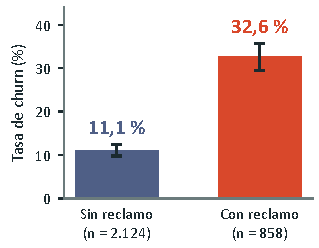
\includegraphics[width=54mm]{f1_reclamo.pdf}\par
    \vspace{0.5mm}
    {\footnotesize\color{muted}\RaggedRight El reclamo casi triplica la tasa de churn.\par}
  \end{columns}
\end{frame}

% =============================================================== 4
\pill{slate}{Fase 2 · Emilia Mortarini}
\begin{frame}{Fase 2: los supuestos del MCO, bajo la lupa}
  \framesubtitle{Modelo diagnosticado: \code{CashbackAmount} sobre los 13 confusores $Z$, en Train ($N = 2.385$).}
  \vspace{1.5mm}
  \begin{columns}[T,onlytextwidth]
    \column{80mm}
    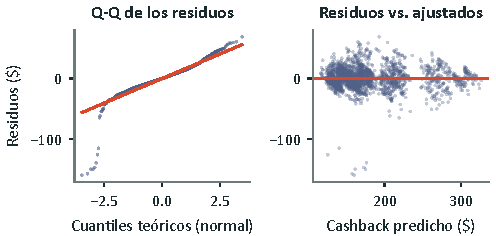
\includegraphics[width=80mm]{f2_residuos.pdf}\par
    \vspace{1.5mm}
    \card[slate]{75.2mm}{PCA ajustado solo en Train}{PC1 explica 19,3\% (intensidad transaccional) y
      PC2 11,7\% (antigüedad vs.\ multi-dispositivo).}

    \column{60mm}
    {\footnotesize
    \renewcommand{\arraystretch}{1.12}
    \begin{tabularx}{60mm}{@{}>{\RaggedRight\arraybackslash}X@{}}
      \toprule
      {\bfseries\color{slate}Homocedasticidad: se viola}\newline
        Breusch-Pagan, $p = 2\cdot10^{-5}$. Se usan errores HC3. \\
      {\bfseries\color{slate}Normalidad: se viola}\newline
        Colas pesadas (Jarque-Bera). Inferencia asintótica. \\
      {\bfseries\color{slate}Independencia: no aplica}\newline
        Durbin-Watson $= 1{,}72$; datos transversales. \\
      {\bfseries\color{slate}Influencia: sin alarmas}\newline
        104 puntos sobre $4/n$ en Cook; 0 con $D > 0{,}5$. \\
      {\bfseries\color{slate}Multicolinealidad: no hay}\newline
        VIF máximo: 3,25. \\
      \bottomrule
    \end{tabularx}}
  \end{columns}
\end{frame}

% =============================================================== 5
\pill{teal}{Fase 3 · Julián Lozano}
\begin{frame}{Fase 3: Random Forest gana el torneo}
  \framesubtitle{Cuatro familias comparadas con validación cruzada solo en Train. Test se evaluó una única vez.}
  \vspace{1mm}
  \begin{columns}[T,onlytextwidth]
    \column{72mm}
    {\small\bfseries ROC-AUC en validación cruzada (5 folds)}\par\vspace{1.5mm}
    \begin{tikzpicture}[x=0.26mm,y=1mm]
      % largo de barra = (AUC - 0,60) * 360
      \foreach \name/\val/\len/\col/\y in {
          Random Forest/0{,}932/119.5/teal/0,
          Logística ElasticNet/0{,}894/105.8/muted/-7.6,
          CART podado/0{,}848/89.2/muted/-15.2,
          Naive Bayes/0{,}786/66.9/muted/-22.8}{
        \node[anchor=east,font=\footnotesize] at (0,\y) {\name};
        \fill[\col,rounded corners=0.6mm] (2,\y-2.5) rectangle (2+\len,\y+2.5);
        \node[anchor=west,font=\footnotesize\bfseries,text=\col] at (3+\len,\y) {\val};
      }
    \end{tikzpicture}\par
    \vspace{1.5mm}
    {\footnotesize\color{muted}\RaggedRight Barras desde 0,60. El AUC fuera de bolsa (OOB) del RF da 0,941:
     coincide con la validación cruzada.\par}

    \column{62mm}
    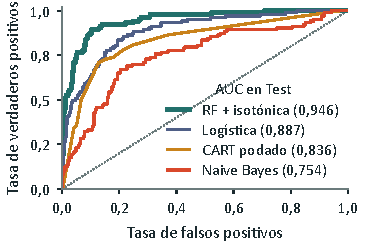
\includegraphics[width=62mm]{f3_roc.pdf}
  \end{columns}
  \vspace{1.5mm}
  \stat[teal]{40.4mm}{12.5mm}{0,946}{ROC-AUC en Test (IC 95\%: 0,922 a 0,968). F1: 0,70.}%
  \hspace{2.7mm}%
  \stat[coral]{40.4mm}{12.5mm}{1,000 → 0,807}{CART sin podar, de Train a Test. Podado: 0,836.}%
  \hspace{2.7mm}%
  \stat[teal]{40.4mm}{12.5mm}{OR 7,0}{Reclamo, en la logística (IC 95\%: 5,1 a 9,6).}
\end{frame}

% =============================================================== 6
\pill{teal}{Fase 3 · Julián Lozano}
\begin{frame}{Fase 3: calibración y la trampa del MDI}
  \framesubtitle{El MDI se calcula en Train y premia a las variables con muchos puntos de corte. La permutación mide la caída real en Test.}
  \vspace{1mm}
  \centering
  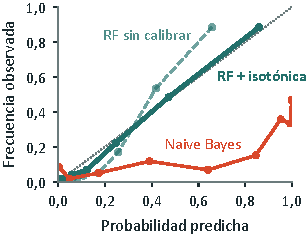
\includegraphics[width=52mm]{f3_calibracion.pdf}\hspace{6mm}%
  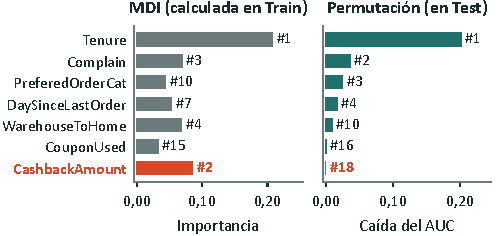
\includegraphics[width=84mm]{f3_importancia.pdf}\par
  \vspace{1.5mm}
  \raggedright
  \stat[teal]{40.4mm}{13.5mm}{0,079 → 0,018}{Error de calibración (ECE) del RF, antes y después de la isotónica.}%
  \hspace{2.7mm}%
  \stat[coral]{40.4mm}{13.5mm}{0,365}{ECE de Naive Bayes: viola la independencia condicional.}%
  \hspace{2.7mm}%
  \stat[coral]{40.4mm}{13.5mm}{\#2 → \#18}{\code{CashbackAmount}: 2.ª por MDI, última por permutación.}
\end{frame}

% =============================================================== 7
\pill{coral}{Fase 4 · Julián y Carola}
\begin{frame}{Fase 4: qué efecto se puede identificar}
  \framesubtitle{$Z$ cierra todos los caminos \emph{backdoor} observables. Ajustar por $M$ o por $C$ sesga la estimación.}
  \vspace{1mm}
  \begin{columns}[T,onlytextwidth]
    \column{76mm}
    \begin{tikzpicture}[
        nd/.style={rounded corners=1.5mm,inner xsep=2.2mm,inner ysep=1.8mm,font=\small\bfseries,align=center},
        ar/.style={-{Stealth[length=2.1mm]},line width=0.55mm,color=ink},
        az/.style={-{Stealth[length=2.1mm]},line width=0.55mm,color=slate},
        au/.style={-{Stealth[length=2.1mm]},line width=0.45mm,color=muted,dashed}]
      \node[nd,fill=amber!75!white]            (T) at (0mm,0mm)    {$T$ · usó cupón};
      \node[nd,fill=okgreen!80!ink,text=white] (Y) at (52mm,0mm)   {$Y$ · churn};
      \node[nd,fill=coral!22!white]            (M) at (26mm,11mm) {$M$ · mediadores};
      \node[nd,fill=slate!25!white]            (Z) at (26mm,25mm)  {$Z$ · 13 confusores};
      \node[nd,fill=amber!22!white]            (C) at (26mm,-15mm) {$C$ · colisionador};
      \node[nd,draw=muted,dashed,text=muted,font=\small] (U) at (26mm,38mm) {$U$ · \emph{engagement}, no observado};
      \draw[ar,line width=0.8mm] (T) -- (Y);
      \draw[ar] (T) -- (M); \draw[ar] (M) -- (Y);
      \draw[az] (Z) -- (T); \draw[az] (Z) -- (Y);
      \draw[ar] (T) -- (C); \draw[ar] (Y) -- (C);
      \draw[au] (U) to[bend right=38] (T.north west);
      \draw[au] (U) to[bend left=38] (Y.north east);
    \end{tikzpicture}

    \column{64mm}
    \card[coral]{59.2mm}{808 clientes sin contrafáctico}{En 6 estratos, el 100\% usa cupón. El efecto se
      estima en los \textbf{2.012} con soporte común.}\par
    \vspace{2mm}
    \card[coral]{59.2mm}{Balance tras ponderar}{$|\mathrm{SMD}|$ máximo: de 0,483 a \textbf{0,107}.}\par
    \vspace{2mm}
    \card[coral]{59.2mm}{Las dos trampas, medidas}{Con el mediador: $-2{,}39$\pp; bloquea el efecto
      indirecto. Con el colisionador: $-0{,}74$\pp; sesgo de Berkson. Ajuste correcto: $-1{,}16$\pp.}
  \end{columns}
\end{frame}

% =============================================================== 8
\pill{coral}{Fase 4 · Julián Lozano}
\begin{frame}{Fase 4: no hay evidencia de retención}
  \framesubtitle{Los cuatro estimadores ajustados incluyen el 0 en su IC 95\%, y las tres refutaciones pasan.}
  \vspace{1mm}
  \begin{columns}[T,onlytextwidth]
    \column{76mm}
    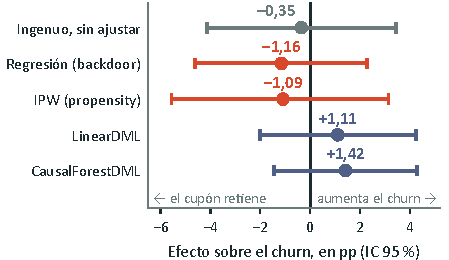
\includegraphics[width=76mm]{f4_forest.pdf}\par
    \vspace{0.5mm}
    {\footnotesize\color{muted}\RaggedRight $N = 2.012$ con soporte común. DoWhy en 4 pasos: modelar,
     identificar, estimar y refutar.\par}

    \column{64mm}
    \begin{tikzpicture}
      \node[rounded corners=1.8mm,fill=tint,inner sep=2.4mm,anchor=north west] (s) {%
        \begin{minipage}[t]{59.2mm}\nosp
        {\small\bfseries Semáforo de refutaciones\par}\vspace{1mm}
        {\footnotesize
        \tikz[baseline=-0.6ex]\fill[okgreen] (0,0) circle (1.2mm);\; Confusor aleatorio: $-1{,}16$\pp\par\vspace{0.5mm}
        \tikz[baseline=-0.6ex]\fill[okgreen] (0,0) circle (1.2mm);\; Tratamiento placebo: $+0{,}09$\pp\par\vspace{0.5mm}
        \tikz[baseline=-0.6ex]\fill[okgreen] (0,0) circle (1.2mm);\; Submuestra del 80\%: $-0{,}99$\pp\par}
        \end{minipage}};
    \end{tikzpicture}\par
    \vspace{2mm}
    \card[coral]{59.2mm}{Sesgo de confusión}{Ingenuo $-0{,}35$\pp\ vs.\ ajustado $-1{,}16$\pp:
      el sesgo es de $+0{,}81$\pp.}\par
    \vspace{2mm}
    \card[coral]{59.2mm}{Dosis y heterogeneidad}{Cada cupón adicional: $+1{,}07$\pp\ de churn
      ($p = 0{,}024$). Ningún segmento con efecto significativo.}
  \end{columns}
\end{frame}

% =============================================================== 9
\pill{amber}{App · Emilia Mortarini}
\begin{frame}{Demo: la decisión en tres pantallas}
  \framesubtitle{La app consume los artefactos auditados: no reentrena modelos en vivo.}
  \vspace{2mm}
  \begin{columns}[T,onlytextwidth]
    \column{40mm}
    {\small\bfseries\color{amber}1 · Diagnóstico y PCA}\par\vspace{1.2mm}
    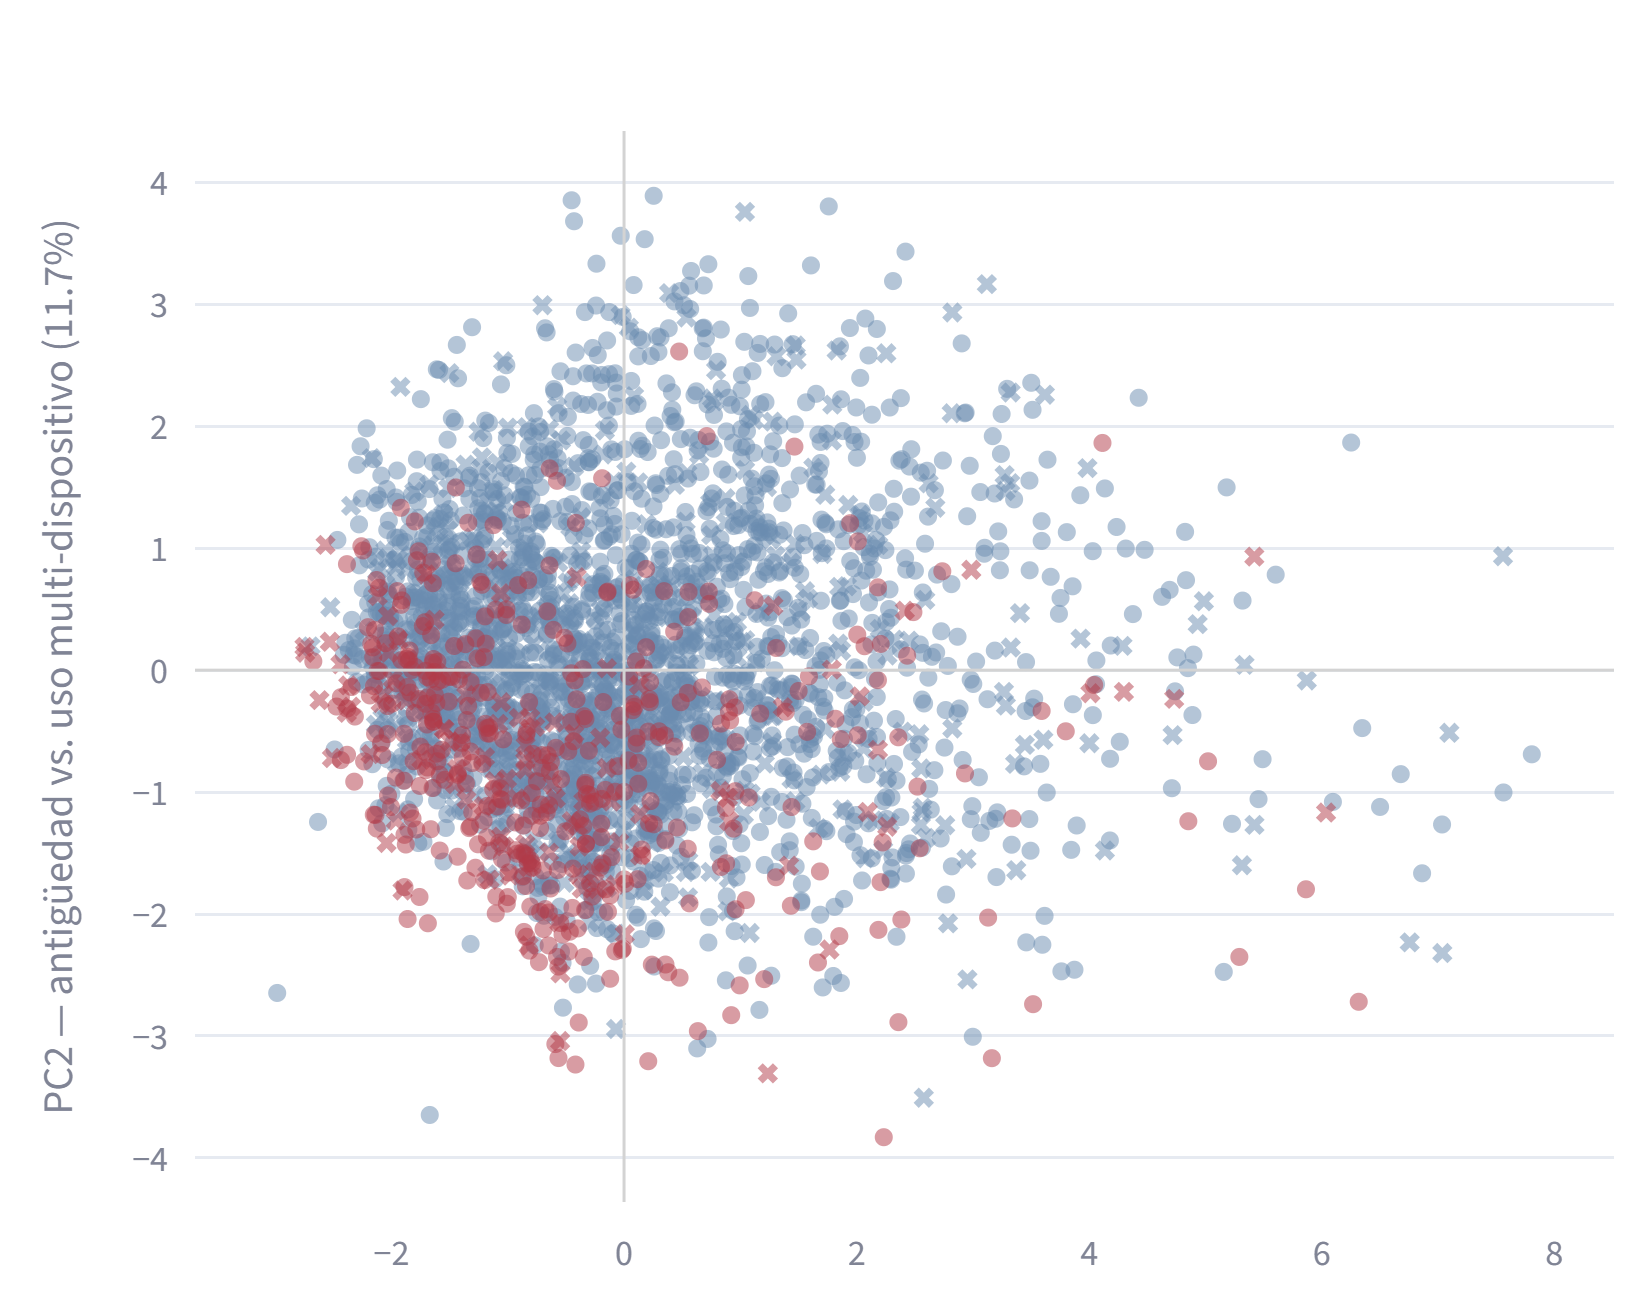
\includegraphics[width=40mm]{app_m1.png}\par\vspace{1.2mm}
    {\footnotesize\RaggedRight Filtros, faltantes y proyección PC1–PC2.\par}
    \column{56mm}
    {\small\bfseries\color{teal}2 · Simulador predictivo}\par\vspace{1.2mm}
    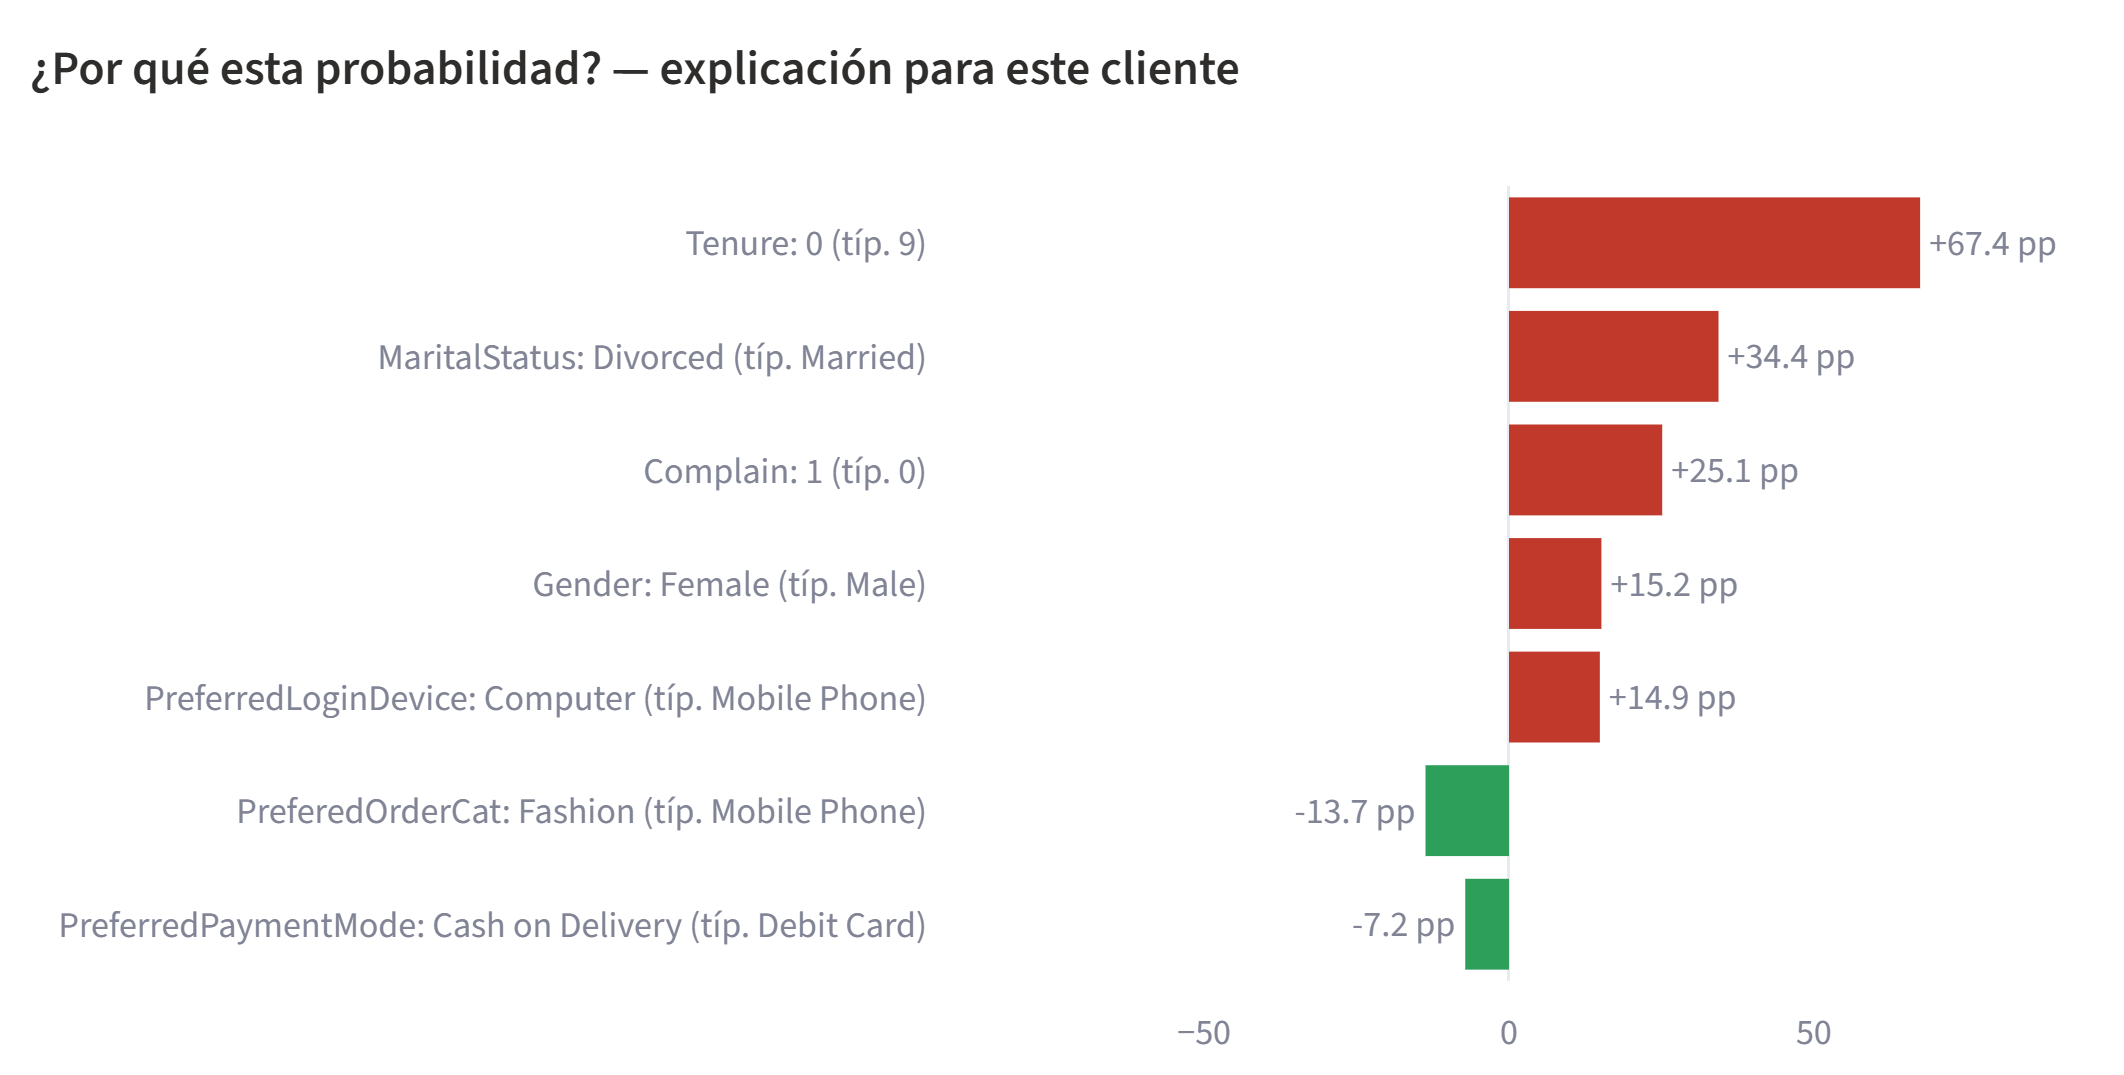
\includegraphics[width=56mm]{app_m2.png}\par\vspace{1.2mm}
    {\footnotesize\RaggedRight Probabilidad calibrada y explicación por cliente. Este perfil:
     71,4\% de churn.\par}
    \column{44mm}
    {\small\bfseries\color{coral}3 · Simulador causal}\par\vspace{1.2mm}
    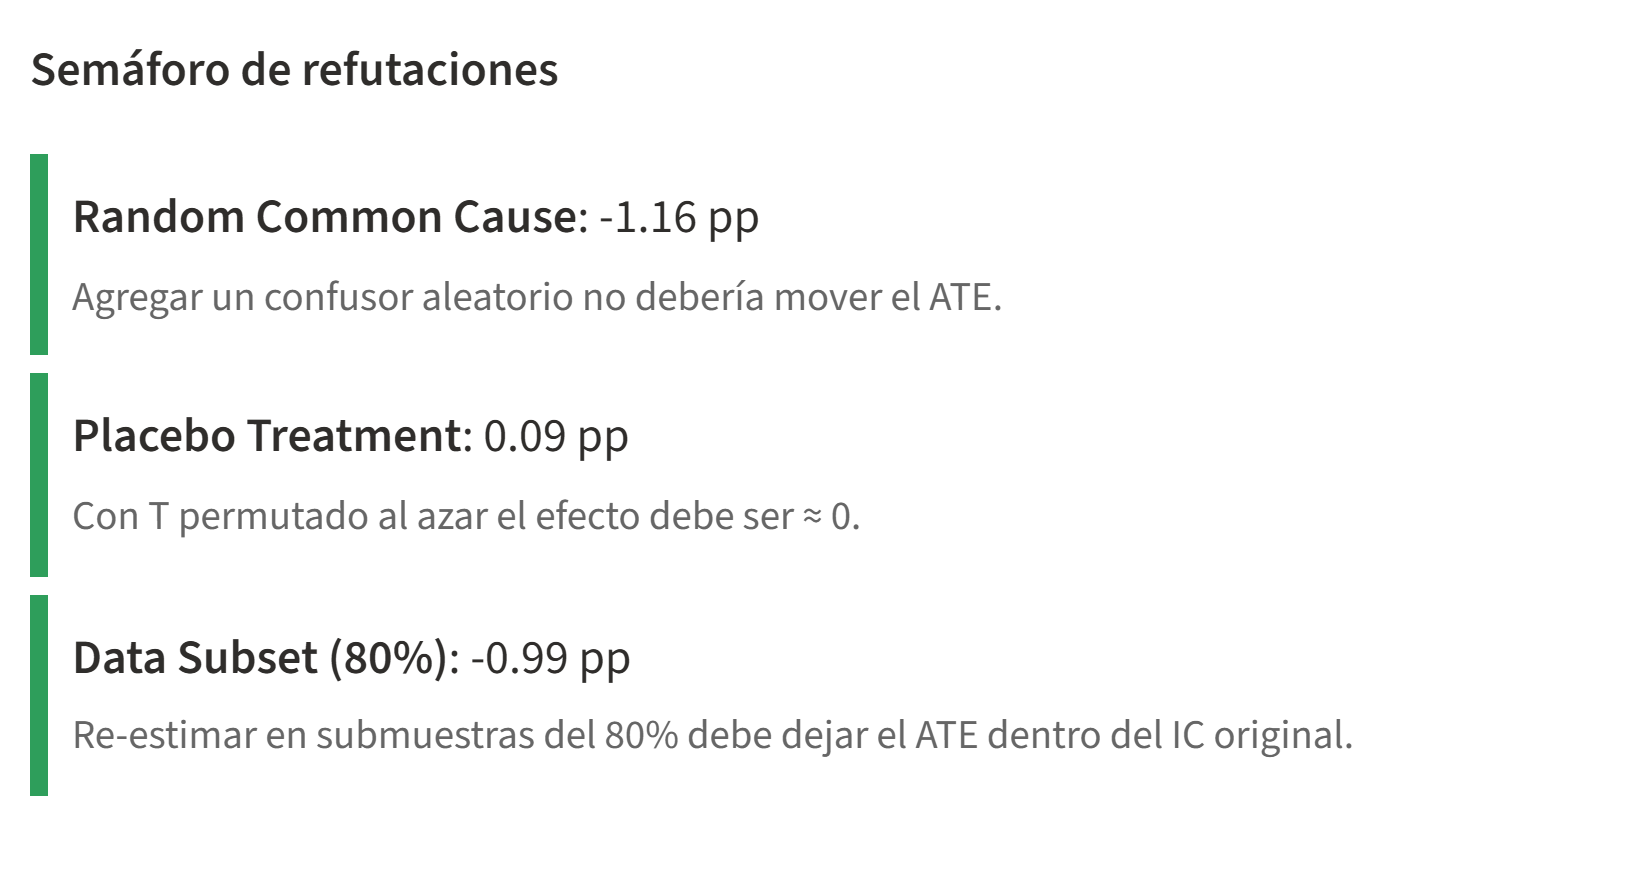
\includegraphics[width=44mm]{app_m3.png}\par\vspace{1.2mm}
    {\footnotesize\RaggedRight DAG, ATE con IC, semáforo de refutaciones y curvas de CATE.\par}
  \end{columns}
  \vfill
  \strip{{\small\bfseries\color{amber}tpi-eamr-grupo-atomos.streamlit.app}\quad en vivo, en Streamlit Community Cloud}
  \vspace{2mm}
\end{frame}

% =============================================================== 10
\pill{amber}{Proceso · Emilia y Carola}
\begin{frame}{Cómo trabajamos: Quality Gate y bitácora}
  \framesubtitle{Ningún cambio entra a \code{main} sin la firma de QA.}
  \vspace{1.5mm}
  \begin{columns}[T,onlytextwidth]
    \column{78mm}
    \begin{tikzpicture}[
        blk/.style={rounded corners=1.6mm,fill=tint,minimum width=35.5mm,inner sep=2mm,align=center,font=\footnotesize},
        arr/.style={-{Stealth[length=1.8mm]},line width=0.45mm,color=muted}]
      \node[blk,fill=amber,text=white] (qg) {\textbf{Quality Gate}\\ruff + pytest\\+ chequeo de \emph{leakage}};
      \node[blk,below=4mm of qg] (src) {\textbf{\code{src/}}\\limpieza, inferencia,\\modelos y causal};
      \node[blk,below=4mm of src] (art) {\textbf{\code{artifacts/}}\\modelo, resultados,\\DAG y CATE};
      \node[blk,right=5mm of src] (nb) {\textbf{Notebook maestro}\\101 celdas, sin errores};
      \node[blk,right=5mm of art] (app) {\textbf{Web App}\\3 módulos, en la nube};
      \draw[arr] (qg) -- (src); \draw[arr] (src) -- (art);
      \draw[arr] (src) -- (nb); \draw[arr] (art) -- (app);
    \end{tikzpicture}

    \column{62mm}
    {\small\bfseries Tres errores que el proceso atajó}\par\vspace{1.5mm}
    \card[amber]{57.2mm}{2.638 copias en el dataset}{Inflaban el AUC a 0,993.}\par
    \vspace{1.8mm}
    \card[amber]{57.2mm}{IPW no reproducible}{Se fijaron el modelo de \emph{propensity} y la semilla.}\par
    \vspace{1.8mm}
    \card[amber]{57.2mm}{\code{CityTier} ignorado en la app}{Hasta 52\pp\ de error. Hoy lo cubre un test.}
  \end{columns}
  \vfill
  \strip{\textbf{Bitácora de 5 entradas:} hipótesis, supuestos, experimentos fallidos, debate causal y uso de IA.}
  \vspace{1.5mm}
\end{frame}

% =============================================================== 11
\begin{darkslide}
\pill{coral}{Conclusiones · Carola Nasif}
\begin{frame}{Detectar con ML, decidir con evidencia causal}
  \framesubtitle{El modelo dice a quién mirar. No dice que un cupón lo retenga.}
  \vspace{3mm}
  \cardh[amber!60!white]{40.4mm}{19mm}{1 · Detectar}{RF con isotónica para priorizar clientes en riesgo. No como gatillo de cupones.}%
  \hspace{2.7mm}%
  \cardh[amber!60!white]{40.4mm}{19mm}{2 · No escalar cupones}{Ningún IC excluye el 0. Cada cupón extra se asocia a más churn.}%
  \hspace{2.7mm}%
  \cardh[amber!60!white]{40.4mm}{19mm}{3 · Experimentar}{Atacar reclamos y primeros meses. Validar el
    cupón con un A/B test.}\par
  \vspace{2.7mm}
  \strip{{\bfseries\color{amber!60!white}Predecir no es intervenir.} \code{Tenure} es la variable n.º 1 y no
    se puede cambiar. El cupón sí, pero es la n.º 16 de 18 y no muestra efecto causal.}\par
  \vspace{2.7mm}
  \strip{{\bfseries\color{amber!60!white}Regla:} el cupón conviene solo si $-\mathrm{ATE}\cdot V > c$.
    Si retener a un cliente vale \$100, debería costar menos de \$4,60, aun en el mejor caso del IC.}
\end{frame}
\end{darkslide}

% =============================================================== 12
\pill{slate}{Respaldo · equipo}
\begin{frame}{Respaldo: límites y métricas completas}
  \framesubtitle{Lo que un diseño observacional no puede resolver, y el detalle del torneo en Test.}
  \vspace{2mm}
  \begin{columns}[T,onlytextwidth]
    \column{64mm}
    {\footnotesize
    \renewcommand{\arraystretch}{1.3}
    \begin{tabularx}{64mm}{@{}>{\RaggedRight\arraybackslash}X@{}}
      \toprule
      {\bfseries\color{slate}Uso, no oferta}\newline
        Medimos que el cliente usó un cupón (TOT), no que se lo ofrecieron (ITT). \\
      {\bfseries\color{slate}Positividad}\newline
        El ATE vale para los 2.012 con soporte común. \\
      {\bfseries\color{slate}Confusor oculto}\newline
        Según su fuerza, el ATE va de $-1{,}75$ a $+6{,}17$\pp. \\
      {\bfseries\color{slate}Datos transversales}\newline
        No se descarta causalidad inversa. \\
      \bottomrule
    \end{tabularx}}

    \column{76mm}
    {\footnotesize
    \renewcommand{\arraystretch}{1.3}
    \begin{tabularx}{76mm}{@{}>{\RaggedRight}X r r r r@{}}
      \toprule
      \textbf{Modelo (Test)} & \textbf{AUC} & \textbf{F1} & \textbf{Brier} & \textbf{ECE} \\
      \midrule
      Naive Bayes          & 0,754 & 0,40 & 0,322 & 0,365 \\
      CART sin podar       & 0,807 & 0,65 & 0,136 & 0,039 \\
      CART podado          & 0,836 & 0,55 & 0,107 & 0,049 \\
      Logística ElasticNet & 0,887 & 0,58 & 0,090 & 0,023 \\
      Random Forest        & 0,943 & 0,69 & 0,072 & 0,079 \\
      \textbf{RF + isotónica} & \textbf{0,946} & \textbf{0,70} & \textbf{0,064} & \textbf{0,018} \\
      \bottomrule
    \end{tabularx}}\par
    \vspace{1.5mm}
    {\footnotesize\color{muted}\RaggedRight Reproducible: semillas fijas y entorno en
     \code{requirements.lock}.\par}
  \end{columns}
\end{frame}

\end{document}
